\subsection{A parametrized example}

Let us consider the following parametrized 
example: $\alpha = \{1 \leq x, x \leq n \}; \beta = \{f(x) = a, 
  f(1) \neq a,
  f(2) \neq a, \dots
  f(n-1) \neq a,
f(n) \neq a\}$ where $n > 1, a$ are fixed integers. We can see that an 
interpolant for this parametrized input problem is 
$x = 1 \lor x = 2 \lor \dots \lor x = n-1 \lor x = n$.

For the case $n = 3, 4, 5$, both the implementation, Z3, and Mathsat were able
to compute the expected result discussed above. This particular test
was useful to check disjunction of equalities propagation mechanism in the
implementation work.

\subsection{Performance evaluation} \label{performance_thcomb}

This section discusses a parametrized problem 
in the EUF + UTVPI theory and compares the times required by
our implementation, iZ3, and Mathsat.

\begin{lemma} \label{performance_test_lemma_thcomb}
  Let $x, a$ be constants and $f$ a unary function 
  in the language of the combined theory of EUF and UTVPI.
  The following conjunction is unsatisfiable for any
  fixed $n \in \mathbb{N}$:
  \begin{equation*}
    1 \leq x \land x \leq n 
    \land f(x) = a 
    \land \bigwedge_{i=1}^{n} f(i) \neq a
  \end{equation*}
\end{lemma}

\begin{proof}
  Using the inequalities $1 \leq x \land x \leq n$
  we can conclude that $x = 1 \lor x = 2 \lor \dots \lor x = n$.
  since we are in the theory of UTVPI for integers.
  We can prove that $x \neq i$ where $i \in \{1, \dots, n \}$.
  Suppose, by contradiction, that $x = i$, so by congruence
  we have that $f(x) = f(i)$, thus $f(i) = a$. This will 
  contradict the conjunction $\bigwedge_{i=1}^{n} f(i) \neq a$.
  Repeating the above step we can prove that 
  $\bigwedge_{i=1}^n x \neq i$. Using $n$ resolution steps, 
  the first disjunction will entail $\bot$ with 
  $\bigwedge_{i=1}^{n} x \neq i$.
\end{proof}

The interpolation pair for our performance test 
is $(1 \leq x \land x \leq n, 
f(x) = a \land \bigwedge_{i=1}^{n} f(i) \neq a)$
for fixed $n \in \mathbb{N}$.
It is easy to see that the pair is inconsistent due to the lemma 
\ref{performance_test_lemma_thcomb}. 

The interpolant in this problem is pretty simple since the 
A-part is already a common conjunction in the language of the
combined theory. For the latter, we tested two versions of our
implementation, one that executes the algorithm proprosed in
this section and the second includes an additional check in 
the algorithm described in this chapter which returns as result
the formula in the A-part if this formula is a conjunction of 
common symbols.

The first experiment tested values for $n$ from $\{2, \dots, 8\}$.
Since the second approach returns a result immediately after
checking if the input is common or not, we tested the parametrized
problem for values in $\{2, \dots, 2500\}$. We show a table and a
graph for the first and second experiments respectively.

\begin{table}[h]
  \centering
  \begin{tabular}{cccc}
    \toprule
    Parameter n        & iZ3 & Mathsat & Our implementation \\
    \cmidrule{2-4}                                          \\
    2 & 0.006 & 0.004 & 0.026    \\
    3 & 0.006 & 0.008 & 0.030    \\
    4 & 0.003 & 0.005 & 0.082    \\
    5 & 0.01  & 0.004 & 0.706    \\
    6 & 0.007 & 0.004 & 11.347   \\
    7 & 0.013 & 0.004 & 213.431  \\
    8 & 0.009 & 0.008 & 5355.216 \\
    \bottomrule
  \end{tabular}
  \caption{Time in seconds obtained for the first experiment.}
\end{table}

\begin{figure}
  \centering
  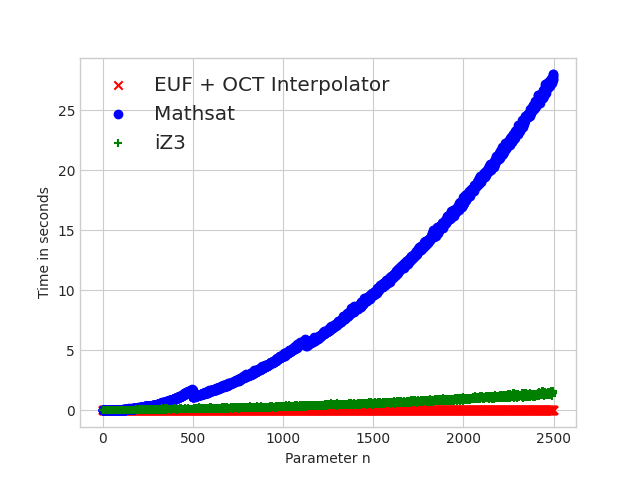
\includegraphics[scale=0.9]{figures/thci_performance_graph_large}
  \caption{Performance comparison graph of EUF + UTVPI 
    interpolant generation
    algorithms for paramatrized problem from section 
  \ref{performance_thcomb}} 
  \label{performance_graph_thcomb}
\end{figure}

%%% Local Variables:
%%% mode: latex
%%% TeX-master: "main"
%%% End:
